% DRAFT. Rewrite the prose in your own words before submission (venue AI policies; see the
% LLM-use statement at the end). Port into the workshop's official style file when the call is out.
\documentclass[10pt]{article}
\usepackage[margin=1in]{geometry}
\usepackage[T1]{fontenc}
\usepackage{lmodern,microtype,graphicx,booktabs,amsmath,multirow}
\usepackage[round]{natbib}
\usepackage[colorlinks=true,linkcolor=black,citecolor=black,urlcolor=blue]{hyperref}
\setlength{\parskip}{0.3em}

\title{Do Interpretability Signals Add Predictive Information About Generalisation?\\
A Pre-registered Test on 100 BERTs}
\author{Pranav Kalla\\[2pt]\small PES University \quad \texttt{kallapranav97@gmail.com}}
\date{}

\begin{document}
\maketitle

\begin{abstract}
\noindent Interpretability measurements computed on in-distribution (ID) data can predict how models behave out of distribution (OOD) in synthetic settings. Whether they tell us anything that cheaper measurements do not is less clear. We test this incremental question on the 100 BERT-base models of \citet{mccoy2020}, which reach near-identical MNLI accuracy but range from 5\% to 55\% on HANS lexical-overlap non-entailment items. Using a frozen 70/30 split of models and a decision rule fixed in advance, we compare head-ablation profiles, attention to repeated words, syntactic-role probes and the convexity-gap loss geometry of \citet{juneja2023} with behavioural, weight-space and representational baselines, all computed without HANS. Every family predicts generalisation on its own (cross-validated $R^2$ 0.27--0.61), but none improves held-out prediction over the baselines. For head ablation and attention, the gain is $-0.012$ $R^2$ (95\% CI $[-0.035, +0.011]$). The strongest single predictor is the models' own behaviour on high-overlap MNLI items. Separately, ablating almost any set of six attention heads lowers HANS accuracy (56 of 60 random sets) while MNLI accuracy changes by under one point. The heads that best predict generalisation are not causally special once their ablation magnitude is controlled for. All results come from one population; the pre-registered test was null-consistent, and the remaining analyses are exploratory.
\end{abstract}

\section{Introduction}
A growing line of work asks interpretability to predict, not only explain: if we understand a mechanism, we should be able to forecast how the model treats inputs it has not seen \citep{li2025,position2026}. \citet{li2025} show that attention patterns observed on ID data predict which generalisation rule each of hundreds of small Transformers follows OOD on synthetic tasks, and call for tests in realistic settings.

Prediction alone does not show that interpretability is useful. Many cheap measurements of a trained model also carry information about its OOD behaviour: its accuracy, its answers on particular ID inputs, its weights, and the geometry of its loss landscape \citep{juneja2023,ding2021}. The question for practice is \emph{incremental}: given what these cheaper measurements already tell us, does looking inside the model add anything?

We study this in a realistic, well-characterised population: the 100 BERT-base models that \citet{mccoy2020} fine-tuned on MNLI with different seeds. These models share architecture, data and ID accuracy, but differ sharply in whether they adopt the lexical-overlap heuristic tested by HANS \citep{mccoy2019}. Our contributions are:
\begin{enumerate}\itemsep0pt
\item a pre-registered, held-out comparison of interpretability signals against behavioural, representational, weight-space and loss-geometry baselines, with every feature computed from non-HANS data (\S\ref{sec:setup});
\item a calibrated test of incremental predictive value. We show that two common alternatives give misleading answers on cross-validated predictions (\S\ref{sec:stats});
\item the finding that no interpretability signal we tested improves on cheap baselines, with bounds tight enough to rule out more than about one point of $R^2$ for the main signals (\S\ref{sec:results});
\item a causal check showing that generalisation in this population is broadly fragile to head ablation, while the heads that best predict it are not special (\S\ref{sec:causal}).
\end{enumerate}

\section{Setup}\label{sec:setup}
\paragraph{Population and outcome.} We use the public checkpoints of \citet{mccoy2020} (\texttt{connectivity/feather\_berts\_0..99}). Our forward passes reproduce the stored predictions (99.85--99.95\% argmax agreement on 5 models) and the reported MNLI matched-dev range (83.7--84.8\%).

The outcome is accuracy on the 5{,}000 HANS lexical-overlap non-entailment items. Across models it has mean 27.7\%, range 5.2--54.5\%, and a between-model SD 19.5 times the binomial sampling SD. Template-blocked split-half reliability is $r=0.96$, so scores are stable. MNLI accuracy alone explains 24\% of the variance across all 100 models.

\paragraph{Pre-registration.} Before computing any feature, we froze a random 70/30 split of models, the feature definitions, the regression method and a decision rule. GO required internal signals to raise held-out $R^2$ over all baselines by at least 0.10 with a 95\% CI above zero. PIVOT applied if internal signals predicted but missed that bar, and STOP if they did no better than MNLI accuracy. The 30 test models were scored once. Everything after that single look is exploratory and labelled as such; the audit trail is in the repository.

\paragraph{Features.} All features use MNLI matched-dev inputs, or unrelated text for the probe; none uses HANS. A fixed probe set holds 256 MNLI pairs with high word overlap (at least 80\% of hypothesis words appear in the premise) and 256 other pairs.
\begin{itemize}\itemsep0pt
\item \emph{Head ablation:} the change in entailment log-odds when each of the 144 heads is mean-ablated, averaged separately over high-overlap and other items.
\item \emph{Attention to repeated words:} per head, the attention mass from hypothesis tokens to identical premise tokens, and to the premise overall.
\item \emph{Syntactic-role probe:} logistic probes on 2{,}000 Universal Dependencies (English EWT) sentences that classify argument roles (subject, object, passive subject, indirect object, oblique) and 12 general relations from head and dependent representations at each layer. The score is selectivity: accuracy minus control-task accuracy \citep{hewitt2019}.
\item \emph{Baselines:}
  \begin{itemize}\itemsep0pt
  \item ID behaviour: accuracy, per-class recall and confidence; and entailment log-odds on each of the 1{,}093 high-overlap MNLI items.
  \item Weight deltas from pretrained BERT: per-block norms and a CountSketch of the delta.
  \item Euclidean weight geometry.
  \item Linear CKA \citep{kornblith2019} at four depths.
  \item Juneja et al.'s convexity-gap (CG) kernel: interpolation-loss barriers between all 4{,}950 model pairs on 512 MNLI items, computed with their protocol. Recomputed on a second item sample, the CG values correlate at $r=0.99$.
  \end{itemize}
\end{itemize}

\paragraph{Regression.} Each family is fitted by kernel ridge regression, with the ridge strength chosen by exact leave-one-out on the training models. Combinations of families are stacked with non-negative weights fitted on leave-one-out predictions.

\section{Testing incremental value}\label{sec:stats}
The natural check, whether predictions from a new feature family correlate with the outcome beyond the baselines' predictions, is easy to get wrong with cross-validated (CV) predictions. We tried two versions and found both invalid.
\begin{itemize}\itemsep0pt
\item \textbf{A parametric partial $F$-test on out-of-fold predictions.} Out-of-fold predictions from a useless feature set are \emph{anti}-correlated with the outcome, an artefact of each training fold's mean, so the test's null distribution is wrong.
\item \textbf{Permuting the new features across models.} This tests whether the features are unrelated to the outcome, not whether they add information beyond the baselines. A redundant copy of a baseline block ``passed'' it with partial $r \approx 0.20$.
\end{itemize}

We therefore compare models directly. In each fold of 20$\times$10-fold CV, the baseline model and the joint model (baselines plus the new family) are both fitted on the training models and scored on the held-out ones. The per-fold reduction in squared error is tested with the corrected repeated $k$-fold $t$-test \citep{bouckaert2004}.

We calibrated this test before applying it. Five pure-noise blocks gave $p=0.62$--$0.84$, so the test is slightly conservative because the stacker pays for useless inputs. Three redundant copies of baseline blocks gave $p=0.45$--$0.50$, as expected. The test therefore measures added \emph{predictive} information, which is the quantity we care about.

\section{Results}\label{sec:results}
\begin{figure}[t]\centering
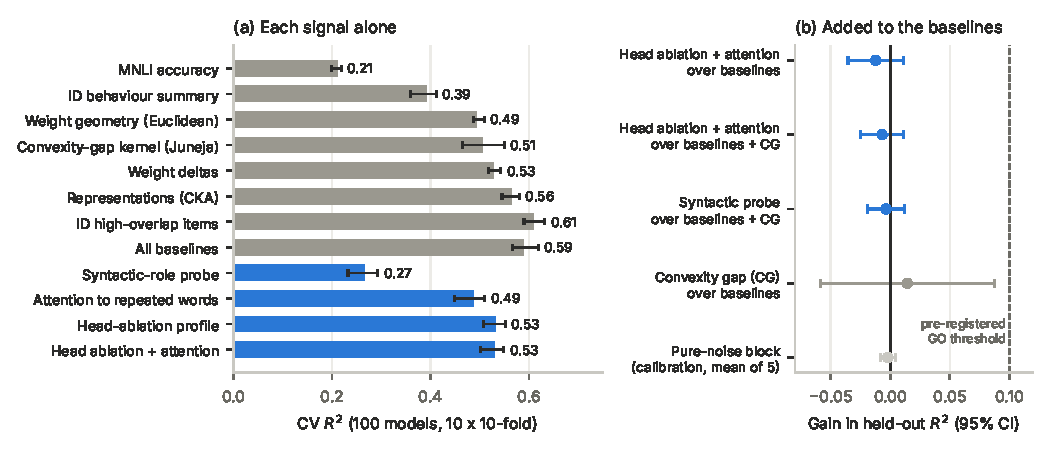
\includegraphics[width=\linewidth]{fig_main.pdf}
\caption{(a) Predictive power of each feature family alone, from 10$\times$10-fold CV over all 100 models (whiskers: 2.5th--97.5th percentile over repeats). Grey: baselines; blue: interpretability signals. (b) Gain in held-out $R^2$ from adding a family to the baselines (nested 20$\times$10-fold CV, corrected $t$-test CIs). The dashed line is the pre-registered GO threshold. ``Baselines'' means all behavioural, weight and representational families; ``CG'' is the convexity-gap kernel.}
\label{fig:main}
\end{figure}

\paragraph{Pre-registered test.} On the 30 held-out models the verdict was PIVOT: internal signals predicted well (test $R^2=0.67$) but did not clear the bar over the baselines (test $R^2=0.69$ with or without them). We report two caveats.
\begin{itemize}\itemsep0pt
\item The pre-registered statistic was degenerate. The stacker gave the internal blocks zero weight, so the difference was exactly zero and its interval collapsed.
\item The test split is atypical. MNLI accuracy correlates $r=0.70$ with the outcome in the test models but $r=0.35$ in the development models, which happens in 2.9\% of random splits. Test $R^2$ values are therefore inflated and not validity estimates.
\end{itemize}
For both reasons we base our conclusions on the analyses below.

\paragraph{Every family predicts; none adds.} Fig.~\ref{fig:main}a shows that each family predicts HANS generalisation on its own. MNLI accuracy is weak ($R^2=0.21$). Weights, CKA, the CG kernel and the internal signals reach 0.49--0.56. The single best predictor is behaviour on high-overlap MNLI items ($0.61$), which is close to an in-distribution measurement of the heuristic itself.

The syntactic probe confirms that roles are encoded: argument-role accuracy is 0.95 at the best layer, against 0.67 on the control task. Its link to generalisation is weaker ($R^2=0.27$) and concentrated in late layers (layer 9: $r=+0.32$).

Fig.~\ref{fig:main}b shows that no family improves held-out prediction once the baselines are included:
\begin{itemize}\itemsep0pt
\item head ablation plus attention: $-0.012$ (95\% CI $[-0.035, +0.011]$);
\item the same, with the CG kernel among the baselines: $-0.007$ $[-0.025, +0.011]$;
\item the syntactic probe: $-0.004$ $[-0.019, +0.012]$.
\end{itemize}
For the interpretability signals, gains above about one point of $R^2$ are excluded, far below the 0.10 we set as practically meaningful. The CG kernel's gain over the baselines is inconclusive ($+0.014$, $[-0.059, +0.087]$).

\paragraph{Reproducing Juneja et al.} With their pipeline (spectral clustering on CG distances, in-sample, all 100 models) we obtain $|r|=0.59$ between their cluster-distance score and HANS-LO accuracy, against their reported 0.67. The value ranges from 0.58 to 0.64 across affinity bandwidths; our bandwidth was fixed before any result. Out of sample, their scalar score reaches CV $R^2=0.32$ and the full CG kernel 0.51.

\section{Causal check: fragile generalisation, unspecial heads}\label{sec:causal}
\begin{figure}[t]\centering
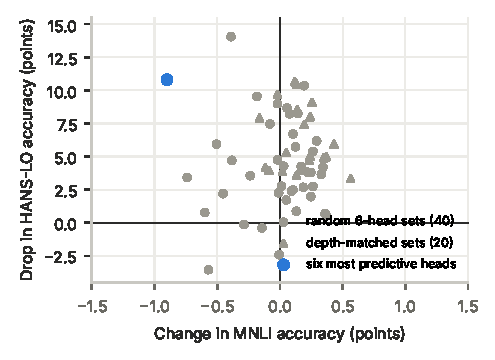
\includegraphics[width=0.55\linewidth]{fig_fragility.pdf}
\caption{Mean effect of mean-ablating six heads on the 30 held-out models. Each grey point is one head set. Almost every set lowers HANS lexical-overlap non-entailment accuracy while leaving MNLI accuracy within $\pm$1 point.}
\label{fig:frag}
\end{figure}

We selected the six heads whose ablation effects correlated most with the outcome on the development models, and mean-ablated them in the 30 held-out models. We compared them with 40 random six-head sets and 20 depth-matched sets, using inference at the level of head sets.

\paragraph{The predictive heads are not special.} The six heads lowered HANS accuracy by 10.8 points, against a median of 3.7 for random sets. This did not reach the pre-stated bar (set-level $p=0.05$ against random sets, $0.10$ on the logit scale, $0.05$--$0.10$ against depth-matched sets). More importantly, these heads have unusually large ablation effects on the development models in general, about four times the typical head. Given that size, their effect on HANS is exactly what we would expect (residual rank $p=0.72$).

\paragraph{Generalisation is fragile.} Across the 60 random and depth-matched sets, 56 lowered HANS accuracy (mean 4.8 points), while MNLI accuracy moved by at most 0.74 points (mean $+0.05$; Fig.~\ref{fig:frag}). The drop on the logit scale does not depend on how well a model generalised (slope $-0.02$). An apparent ``best generalisers lose most'' pattern on the raw-accuracy scale is a floor effect. Removing generic computation thus pushes models toward the heuristic, while ID accuracy is preserved. This fits the view that the heuristic is a default and generalisation is a less robust addition \citep{bhaskar2024}. Our evidence is descriptive and does not identify the mechanism.

\section{Related work}
\citet{li2025} predict OOD rules from attention patterns on synthetic tasks. In their v4 they compare against a hyperparameter baseline, with mixed results, and find that predictive heads need not be causal. We test the incremental question in a realistic population, against baselines measured on the trained models. Our causal result agrees with theirs that prediction and causal specificity come apart.

\citet{mccoy2020} documented the variation we predict. \citet{ding2021} used the same population and outcome to benchmark representational similarity measures. \citet{juneja2023} linked it to linear-connectivity basins, and \citet{brown2023} localised the generalising/heuristic divergence to late layers, consistent with our probe's layer profile. \citet{bhaskar2024} found shared heuristic-core heads in pruned BERT subnetworks. \citet{andriushchenko2023} found sharpness measures uninformative on this population. Work on predicting per-input correctness from internals \citep{huang2025} addresses a different question from our per-model prediction.

\section{Limitations}
\begin{itemize}\itemsep0pt
\item \textbf{One population.} We attempted a second (the 100 QQP BERTs of \citet{juneja2023}, evaluated on PAWS), but its outcomes failed our pre-set reliability gate: almost all models fail almost all PAWS items. We found no other public population with released weights and a reliable OOD outcome.
\item \textbf{A narrow set of signals.} We tested four interpretability signals; others, such as sparse-autoencoder features or circuit discovery, might behave differently.
\item \textbf{A strong behavioural baseline.} Our best baseline is close to an in-distribution measurement of the heuristic itself. That is the point of the comparison, but it makes ``behaviour wins'' less surprising.
\item \textbf{Mostly exploratory evidence.} The only confirmatory test had a degenerate statistic. All other results are exploratory on a population whose test models had already been seen. We report every analysis we ran, including two invalid tests that we replaced.
\end{itemize}

\section{Conclusion}
In a realistic population of 100 fine-tuned BERTs, every interpretability signal we tested predicts which models generalise, but none tells us more than a cheap behavioural probe does. Gains above about one point of $R^2$ are ruled out for the main signals. Interpretability's value for forecasting generalisation should therefore be judged by its \emph{incremental} information, against strong behavioural baselines, with calibrated tests. On that standard, the evidence here is negative.

\paragraph{Reproducibility.} Code, Kaggle and Colab notebooks, all reports, and an audit of every contact with the held-out models are available from the author on request.

\paragraph{LLM-use statement.} The author used an AI assistant (Claude, Anthropic) for code, statistical analysis, literature search and drafting. Independent AI reviewers were used to audit the design, and they found several of the errors reported in \S\ref{sec:stats} and the audit. All design decisions, claims and the final text are the author's responsibility.

\bibliographystyle{plainnat}
\begin{thebibliography}{14}\small\itemsep0pt
\bibitem[Andriushchenko et~al.(2023)]{andriushchenko2023} M.~Andriushchenko, F.~Croce, M.~M\"uller, M.~Hein, N.~Flammarion. A modern look at the relationship between sharpness and generalization. ICML 2023.
\bibitem[Bhaskar et~al.(2024)]{bhaskar2024} A.~Bhaskar, D.~Friedman, D.~Chen. The heuristic core: Understanding subnetwork generalization in pretrained language models. ACL 2024.
\bibitem[Bouckaert and Frank(2004)]{bouckaert2004} R.~R.~Bouckaert, E.~Frank. Evaluating the replicability of significance tests for comparing learning algorithms. PAKDD 2004.
\bibitem[Brown et~al.(2023)]{brown2023} D.~Brown, C.~Godfrey, N.~Konz, J.~Tu, H.~Kvinge. Understanding the inner workings of language models through representation dissimilarity. arXiv:2310.14993, 2023.
\bibitem[Ding et~al.(2021)]{ding2021} F.~Ding, J.-S.~Denain, J.~Steinhardt. Grounding representation similarity with statistical testing. NeurIPS 2021.
\bibitem[Hewitt and Liang(2019)]{hewitt2019} J.~Hewitt, P.~Liang. Designing and interpreting probes with control tasks. EMNLP 2019.
\bibitem[Huang et~al.(2025)]{huang2025} J.~Huang et~al. Internal causal mechanisms robustly predict language model out-of-distribution behaviors. arXiv:2505.11770, 2025.
\bibitem[Juneja et~al.(2023)]{juneja2023} J.~Juneja, R.~Bansal, K.~Cho, J.~Sedoc, N.~Saphra. Linear connectivity reveals generalization strategies. ICLR 2023.
\bibitem[Kornblith et~al.(2019)]{kornblith2019} S.~Kornblith, M.~Norouzi, H.~Lee, G.~Hinton. Similarity of neural network representations revisited. ICML 2019.
\bibitem[Li et~al.(2025)]{li2025} V.~R.~Li, J.~Kaufmann, T.~Qin, M.~Wattenberg, D.~Alvarez-Melis, N.~Saphra. Can interpretation predict behavior on unseen data? arXiv:2507.06445, 2025 (BlackboxNLP 2026).
\bibitem[McCoy et~al.(2019)]{mccoy2019} R.~T.~McCoy, E.~Pavlick, T.~Linzen. Right for the wrong reasons: Diagnosing syntactic heuristics in natural language inference. ACL 2019.
\bibitem[McCoy et~al.(2020)]{mccoy2020} R.~T.~McCoy, J.~Min, T.~Linzen. BERTs of a feather do not generalize together: Large variability in generalization across models with similar test set performance. BlackboxNLP 2020.
\bibitem[Biderman et~al.(2026)]{position2026} Stella Biderman, Mohammad Aflah Khan, Niloofar Mireshghallah, Catherine Arnett, Fazl Barez, and Naomi Saphra. Position: Don't just ``fix it in post'': A science of AI must study training dynamics. arXiv:2606.06533, 2026.
\end{thebibliography}
\end{document}
